\cleartooddpage[\thispagestyle{empty}]
\chapter{Dark Matter}

\section{Evidence for Dark Matter}

Peering out into space, there are affects attributed to dark matter on several different length scales.
As dark matter, by definition, does not directly interact with electromagetic light, most of the evidence for dark matter relies on a combination of gravtiational effects pulling on electromagnetic emitters, and mass distorting the spacetime paths taken by passing light.

On the smallest scales, groups of several thousand stars can be seen revolving around their center of mass, at a larger distribution of speeds than one would expect from the existing visible amount of matter.
At larger scales the optical light from galaxies, as well as hydrogen lines, can be used to measure the amount of mass and its rotational velocity around the center of galaxies.
At even larger scales, galaxy velocities can be measured and compared, x-ray telescopes can monitor the amount of hot gas, and mass-heavy areas of space will gravitationally lens background galaxies.
At the the largest scales, the measurement of oscillations in the cosmic microwave background can be used to determine the amount of dark and baryonic matter.


\subsection{Dwarf Galaxy Scale}
% 10^19m comes from: 
% fornax dwarf spheroidal galaxy wiki page
%    17' x 12.6' in solid angle, call it 15'
%    140kpc away  
%    140kpc * Tan(15') = 0.6kpc = 1.8*10^19m ~ 10^19m
At scales of $\nicetilde 10^{19}$m, groups of thousands stars, called satellite galaxies or dwarf galaxies, lie at the edge of the Milky Way galaxy.
Telescopes can measure the individual spectra of these stars, allowing for their velocity to be calculated.
Often, these observations focus on the Red Giant stars within these dwarf galaxies\cite{dwarf_gal_red_giant}.
By looking at the distribution of these velocities, the total mass of the dwarf galaxy can be inferred.


\subsection{Galaxy Scale}
%
% galaxy rotation curve wiki page, M33 has curve measurements out to 50,000ly
%   50,000ly = 4.7*10^20m ~ 10^20m
At scales of $\nicetilde 10^{20}$m, the effects of Dark Matter on galaxies are observable.
In one method, the total amount of light produced by a quadrant of a galaxy is measured with telescopes.
Known mass-to-light ratios can then be used to calculate the total amount of mass within that quadrant.
This was the earliest method of measuring the mass of a galaxy, producing a low value for the amount of mass.

In a second method, a galaxy's emission spectrum is observed at many positions around its disk (center, outer edges, etc).
By comparing the orientation of the disk with the doppler-shifted position of common spectral lines, one can calculate the average velocity that each chunk is travelling at around the center of the galaxy.
Newton's law of gravity can then be used to calculate the mass contained within a sphere of that same radius.
This calculation ends up with a larger amount of mass.

\subsection{Galaxy Cluster Scale}
%
% galaxy cluster wiki page
% 2-10 Mpc, call it 6Mpc = 1.85*10^23m ~ 10^23m
At scales of $\nicetilde 10^{23}$m, Dark Matter's effects on galactic clusters becomes observable by comparing three techniques.
In the first method, galaxy clusters are be massive enough to bend the images of background galaxies.
The type and amount of bending can be used to determine the mass of the intermediate galaxy.

X-Ray observations of galaxy clusters can measure the amount of hot baryonic mass.
This has been shown distinctly in the Bullet Cluster\cite{bullet}.
In this cluster, the total (baryonic+dark) mass was traced using gravitational lensing of background light.
The baryonic mass was then traced with x-rays, which are emitted by ionized gas in the region.
Figure \ref{fig:bullet} then shows these two masses overlayed.

\begin{figure}[h]
  \begin{center}
    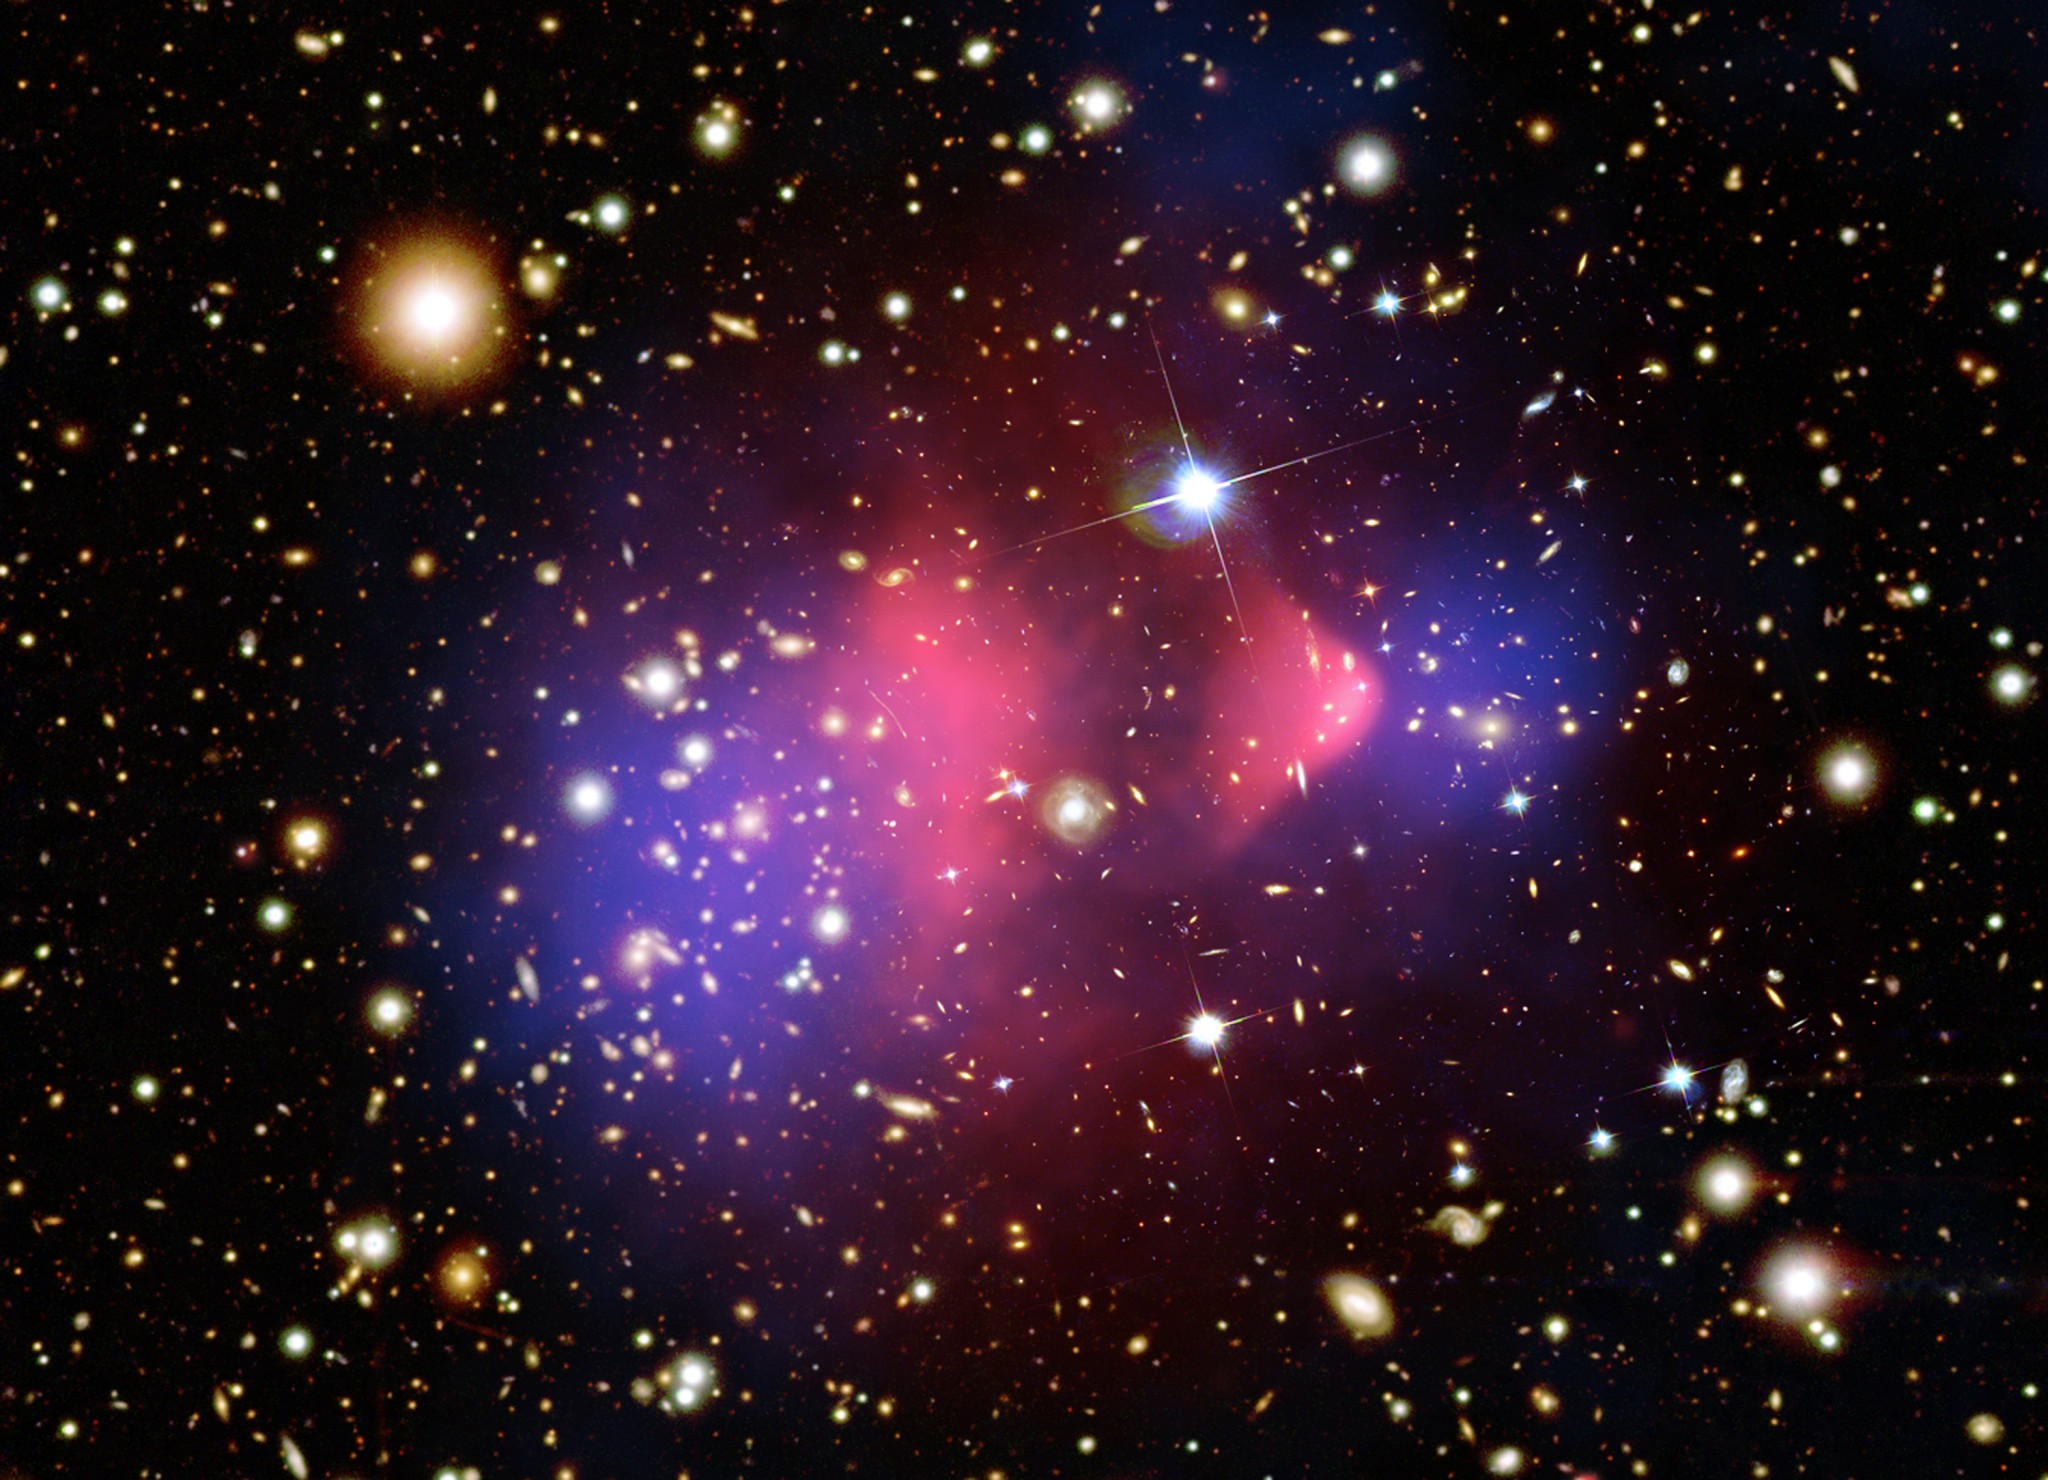
\includegraphics[width=0.95\textwidth]{images/bulletcluster.eps}
    \caption[The Bullet Cluster]{The bullet cluster\cite{bullet_cluster_combined_image}.  The blue clouds indicate the graviational lensing mass\cite{bullet_cluster}, the red represents two clouds of ionized baryons emitting x-rays\cite{bullet_cluster_chandramap}.  The remaining stars and galaxies are imaged in the optical spectrum\cite{bullet_cluster_composite}.}\label{fig:bullet}
  \end{center}
\end{figure}

Followup studies have also been done of other galaxy clusters.
more??


In the second method, the velocity of different galaxies in a cluster can be measured.
By comparing the velocities of different galxies in a cluster, the contained mass within the cluster can be measured.

%\subsection{Inter-Cluster Scale}
% fast radio burst galaxy at z = 0.492 (http://www.nature.com/nature/journal/v530/n7591/full/nature17140.html)
% redshift to distance : d = z c / Ho (http://m.teachastronomy.com/astropedia/article/Relating-Redshift-and-Distance)
% wmap hubble constant = 70.4 (km/s)/Mpc (http://map.gsfc.nasa.gov/universe/bb_tests_exp.html)
% c = 2.99*10^8 m/s = 2.99*10^5 km/s
% 0.492 * 2.99*10^5 km/s / 70.4(km/s)/Mpc = 2089 Mpc = 6.44*10^25 m
%?? NATURE PAPER IS IN QUESTION ??
%At even larger scales of $\nicetilde 10^{25}$m, fast radio bursts and their frequency dispersion can be used to place limits on the amount of baryonic matter in the path of the burst.
%This in turn allows for upper limits to be placed on the amount of dark matter present as well.


\subsection{Universe Scale}
%
% age of universe (13.82*10^9 years * speed of light) = 1.307*10^26m
At the largest scale of the universe, $\nicetilde 10^{26}$m, the cosmic microwave background (CMB) has been used to measure the total amount of dark matter in the universe.
By looking at the structure of the CMB, earlier times in the universe can be studied.
Closer to the big bang, there was a point in time referred to as the 'freezout'.
Before that time, the universe was a sea of quark plasma and other particles, and the temperature was too hot to allow baryons exist for any long period of time.
After that freezout time, the temperature low enough that baryons stopped being created and annihilated.
Thus, the number of baryons that were in the universe at the freezout temperature determines how many baryons are in existance today, since there aren't any significant ways to destroy universe-scale quantities of baryons.
This freezout left an imprint of its structure, where more baryons in some places created more CMB photons, and other places had less of each.
So, by looking at this CMB structure, the total number of baryons in the universe can be measured.



\section{Dark Matter and the Standard Model}

The current paradigm of particle physics is called the Standard Model.
It describes the masses and crosssections of quarks and leptons, as well as how bosons mediate interactions between these particles.
In cosmology, the equivalent of the standard model is $\Lambda$CDM (Lambda Cold Dark Matter). 
$\Lambda$CDM describes how the universe evolved from the big bang, including the contributions of dark matter and dark energy.
It also describes how a non-relativistic (cold) dark matter particle is necessary for the current evolution of the universe.
However, either through wrong mass, wrong quantity, wrong cross section, or wrong velocity, no Standard Model particles can be cold dark matter.
This fuels suspicion than there are new, as of yet unknown particles that can fufill this role.
The two currently favored candidates are WIMPs (the subject of this thesis), and Axions.


\subsection{WIMPs}

WIMPs, or Weakly-Interacting Massive Particles, are predicted to only interact gravitationally and through weak interactions.
A major reason they are a popular dark matter candidate is due to the "WIMP Miracle".
The WIMP miracle is that the dark matter particle's predicted weak force cross section from particle physics is the same order of magnitude as predicted by cosmology.

In particle physics, a WIMP dark matter candidate would need to be around 100GeV, meaning it would have a crosssection around ?? $cm^{2}$.
In cosmology, the early expansion of the universe had an epoch where the dark matter particles froze out, where the universe was large enough that dark matter collisions became infrequent, leading to no new dark matter particles.
The time when this freezout occurred left an imprint on the Microwave Cosmic Background, which can be used to infer the cross section of the dark matter particle, which is around ?? $c^{2}$.

The fact that particle physics predicts ??$cm^{2}$, and cosmology predicts ??$cm^{2}$, is the miracle.
That two separate fields of physics end up predicting a similar dark matter cross section is highly suggestive, and is why many DM studies are devoted to the search for WIMPs.


\subsection{Axions}

Another possible dark matter candidate is the axion.
Originally theorized as a way to solve the strong CP problem ??, they also ended up being a good dark matter candidate.

Most searches for axions consist of looking for changes in photon opacity in the presence of magnetic fields.
This can occur in Earth laboratories, where a laser is shined through a strong magnetic field at an opaque wall (like several meters of concrete), then measuring the number of photons detected on the other side of the wall in a similar magnetic field.
If axions are present, the laser photons will convert into axions in the presence of the magnetic field, pass through the wall, and convert back into photons again on the other side.

In astrophysical scales, this can be done by examining distant galaxies.
Due to the haze of particles in between galaxies, most photons from distant galaxies is lost due to interactions.
If axions are present, extremely distant galaxies that are normally too dim may become detectable.


\subsubsection{Other Potential Candidates}

Other potential ideas that could explain Dark Matter's effects are Massive Compact Halo Objects, or MACHOs.
While WIMPs and Axions are particle-scale dark matter candidates, MACHOs are instead stellar-scale candidates.
These could be either large planets that weren't quite big enough to start fusing hydrogen, or primordial black holes.
Primordial black holes are predicted to have been created shortly after the big bang.
As there is presently no known mechanism for reducing their numbers, the majority of these black holes would be capable of surviving to the present time.

In either case, as these halo objects would be neither strongly absorptive or emissive at any electromagnetic frequency, they would be difficult to detect.
Most theories invovlving MACHOs are constrained by measurements of the universe's total baryonic mass from the measurements of the CMB.
Star-Star gravitational lensing can in principle be used to detect these compact objects, but this technique is difficult and has large systematic errors (macho survey citation??).
While there are significant constraints\cite{pbh_highly_constrained}, primordial black hole mergers can in principle be detected with graviational wave detectors like LIGO\cite{dm_with_ligo}, though at present more observation time is needed.



\section{Dark Matter Search Techniques}


There are three categories of searches for dark matter particles.
Direct Detection experiments attempt to discern when a dark matter particle directly strikes a volume of detection mass, stored deep underground.
Indirect Detection experiments attempt to look for secondary products of dark matter interactions, usually through astrophysical searchs.
Collider searches attempt to produce a dark matter particle through controlled collisions of standard model particles.

% direct
Direct searches consist of an interaction mass, surrounded by light, heat, and acoustic sensors, usually buried deep underground.
These sensors attempt to detect a signal from when a particle strikes the enclosed interaction mass, and discern how much mass and energy the incident particle had.
Most of these detectors are either solid blocks of ??, or liquified gasses like Xenon.

% collider
Collider searches involve accelerating particles in particle accelerators, smashing them together, and searching the resulting explosion of particles for evidence of dark matter particles.

% indirect
Indirect searches involve observing regions of space with telescopes, either looking for secondary particles that may have been produced by a dark matter collisions, or for gravitational effects, like lensing.
The analysis described later in this thesis is an indirect search, examining whether gamma rays near the galactic center match the given predicted shape of a dark matter halo.
Much of the evidence for dark matter, as detailed in section ??, comes from indirect searches.



\section{Mass and Cross-section}


\section{Halo Structure}
Numerical simulations have been performed to simulate the structure of dark matter halos.
On galactic scales, these halos can be modeled with several different density profiles.
Three of the primary profiles are the Burkert, the Einasto, and the Zhao profile.
Each profile describes the mass/volume density of dark matter at a distance r from the halo center.

A Burkert profile (\cite{burkertprofile}) has the form

$ \rho_{DM} \left( r \right) = \frac{ \rho_o r_o3}{ \left( r + r_o \right) \left( r^2 + r_o^2 \right)} $ \label{eqn:burkert}

where $r_o$ is the scale radius of the halo, and $\rho_o$ is the scale density, the density at the scale radius.

The Einasto profile (\cite{einastoprofile1},\cite{einastoprofile2}) has the form

$ \rho_{DM} \left( r \right) = Exp \left( - \frac{2}{\alpha} \left( {\left( \frac{r}{r_o} \right)}^{\alpha} - 1 \right) \right)$ \label{eqn:einasto}

The Zhao profile (\cite{zhaoprofile}) has the form

$ \rho_{DM} \left( r \right) = \frac{\rho_o}{ {\left( \frac{r}{r_o} \right)}^{\gamma} {\left( 1 + {\left( \frac{r}{r_o} \right)}^{\alpha} \right)}^{ \left(\beta - \gamma \right) / \alpha} } $ \label{eqn:zhao}

where $\gamma$ is the slope of the density profile when $r << r_o$, $\beta$ is the slope when $r >> r_o$, and $\alpha$ determines how large the transition region is between $\gamma$ and $\beta$.
A larger $\alpha$ means a smaller transition region.

These profiles can then be used to calculate the spatial distribution of gamma-rays.
For annihilating dark matter, $\rho\left(r\right)^2$ must be integrated along the line of sight.

$ \frac{d\Phi}{dE d\Omega}= \frac{ \left \langle \sigma v \right \rangle }{8 \pi m_\chi^2} \frac{dN}{dE} \int \rho^2 dl $ \label{eqn:dmflux}

?? equation also depends on if particle is symmetric? 8 $\pi$ may change or something ??



